\subsection{Problem Definition}

Define a pattern $P$ to be an $n_{R} $ by $n_{C}$ grid of black and white squares. Let $n = n_R + n_C$.
%See Fig.~\ref{fig:example_pattern} for an example of a pattern.

%\begin{figure}[h]
%\centering
%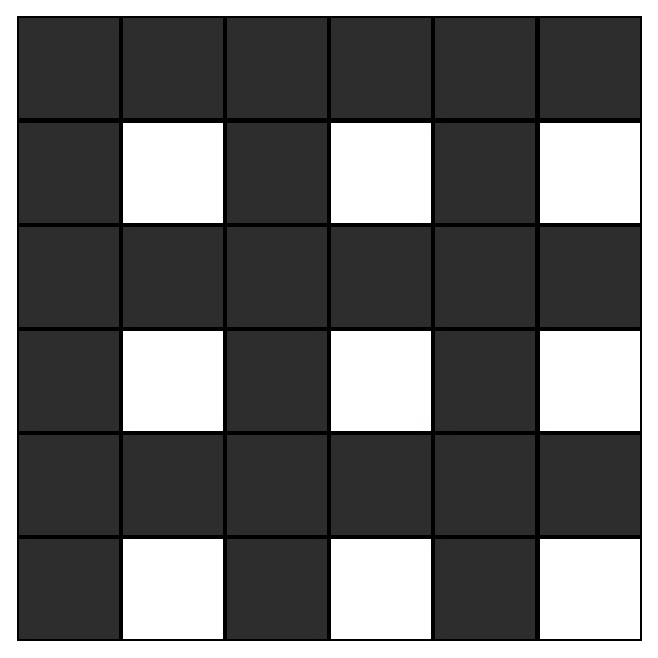
\includegraphics[width=3cm]{example_pattern}
%\caption{An example of a black and white pattern}
%\label{fig:example_pattern}
%\end{figure}

A rectangle strip-rule on $P$ is either a black or white rectangle that extends from one side of the pattern to the opposite side.
Precisely, a rectangle in $P$ is either a set of contiguous rows of $P$ or a set of contiguous columns of $P$.

A rectangle strip-rule list (a SRRL) that generates $P$ is an ordered list of rectangle strip-rules, that when applied in order to a blank (white) grid the size of $P$ creates the target pattern. See Fig.~\ref{fig:pattern_generation} for an example of a pattern generated by a SRRL.

\begin{figure}[h]
\centering
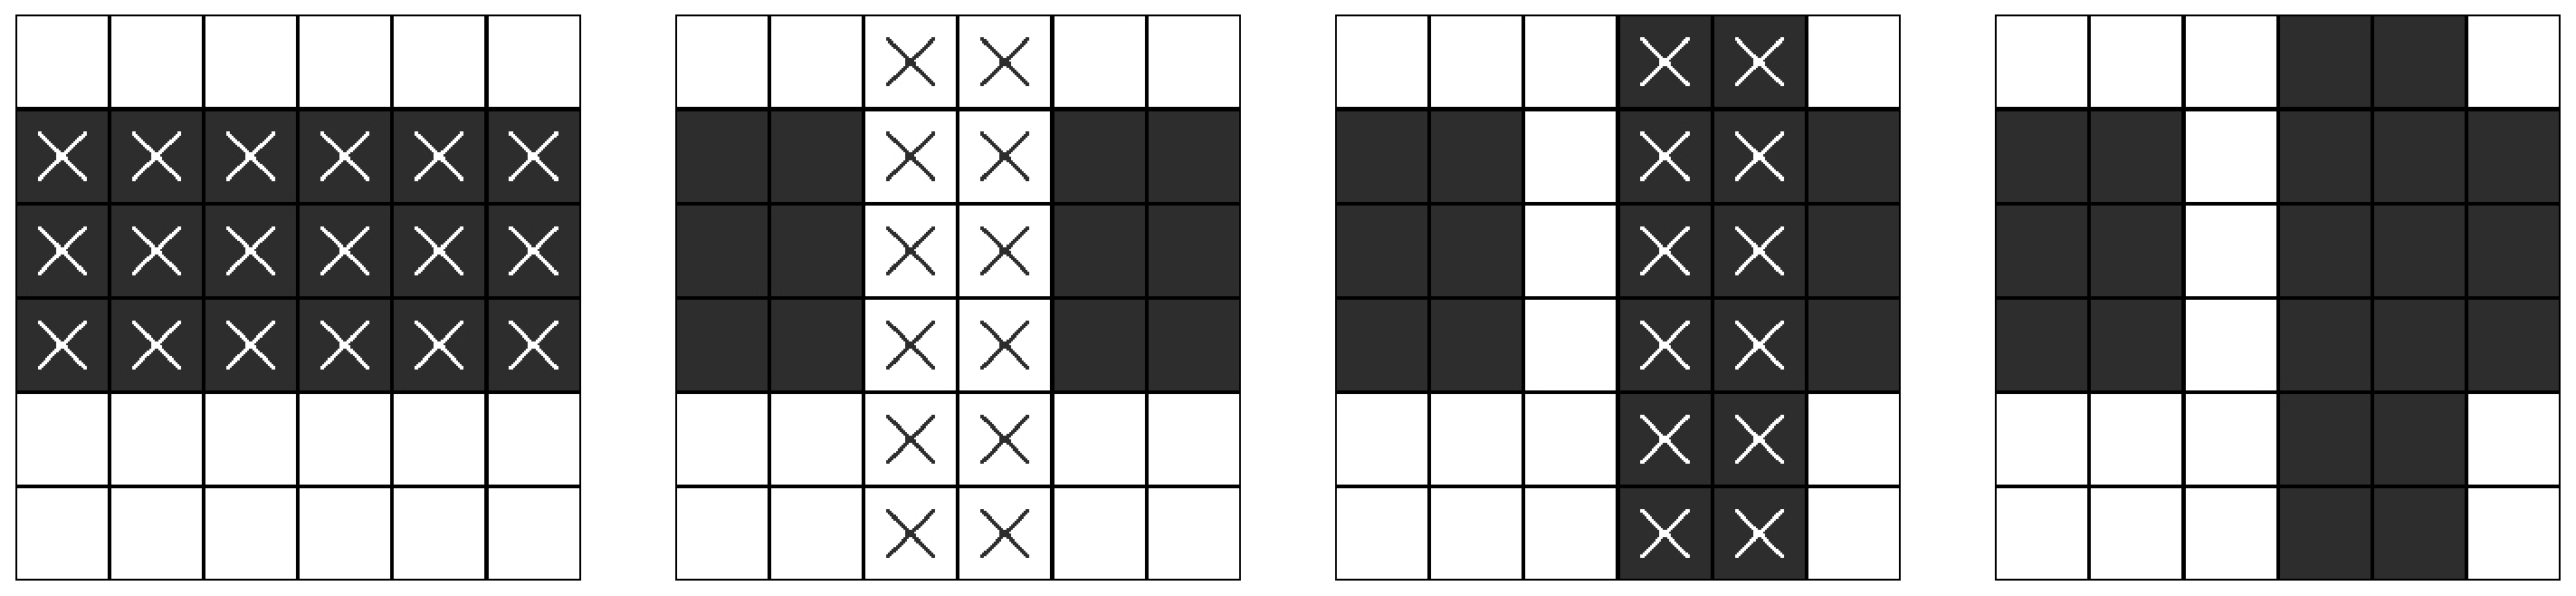
\includegraphics[height=3cm]{pattern_generation}
\caption{A pattern generated by a SRRL of 3 elements.}
\label{fig:pattern_generation}
\end{figure}

We say a pattern $P$ is a strip-rule pattern if there is a SRRL that generates $P$. Note that not every pattern $P$ is a strip-rule pattern. See Fig.~\ref{fig:checkerboard} for an example of a pattern that is not a strip-rule pattern.

\begin{figure}[h]
\centering

\includegraphics[width=1.5cm]{checkerboard}
\caption{The $2 \times 2$ checkerboard: an example of a pattern that is not a strip-rule pattern.}
\label{fig:checkerboard}
\end{figure}

% Our goal on this paper is, given a pattern $P$ of dimensions $n_{R} \times n_{C}$, finding if $P$ is a strip-rule pattern and, if so, finding a minimal SRRL for it.

An SRRL is considered optimal if it has the minimum number of rectangle strip-rules of any SRRL that generates $P$.
